\section{Theoretische Grundlage}
\label{sec:Theorie}
Ziel des Versuches ist es die Totzeit, die Nachentladung sowie Charaketristik eines Geigermüllerzählrohr zu bestimmen.

\subsection{Aufbau eines Geiger-Müller-Zählrohr}
Ein Geiger-Müller-Zählrohr ist ein Messgerät zur Bestimmung von Ionisiernder Strahlung. Ein Modell eines Geiger-Müller-Zählrohr ist in Abbildung \ref{fig:skizze} zu sehen. 
\begin{figure}
  \centering
  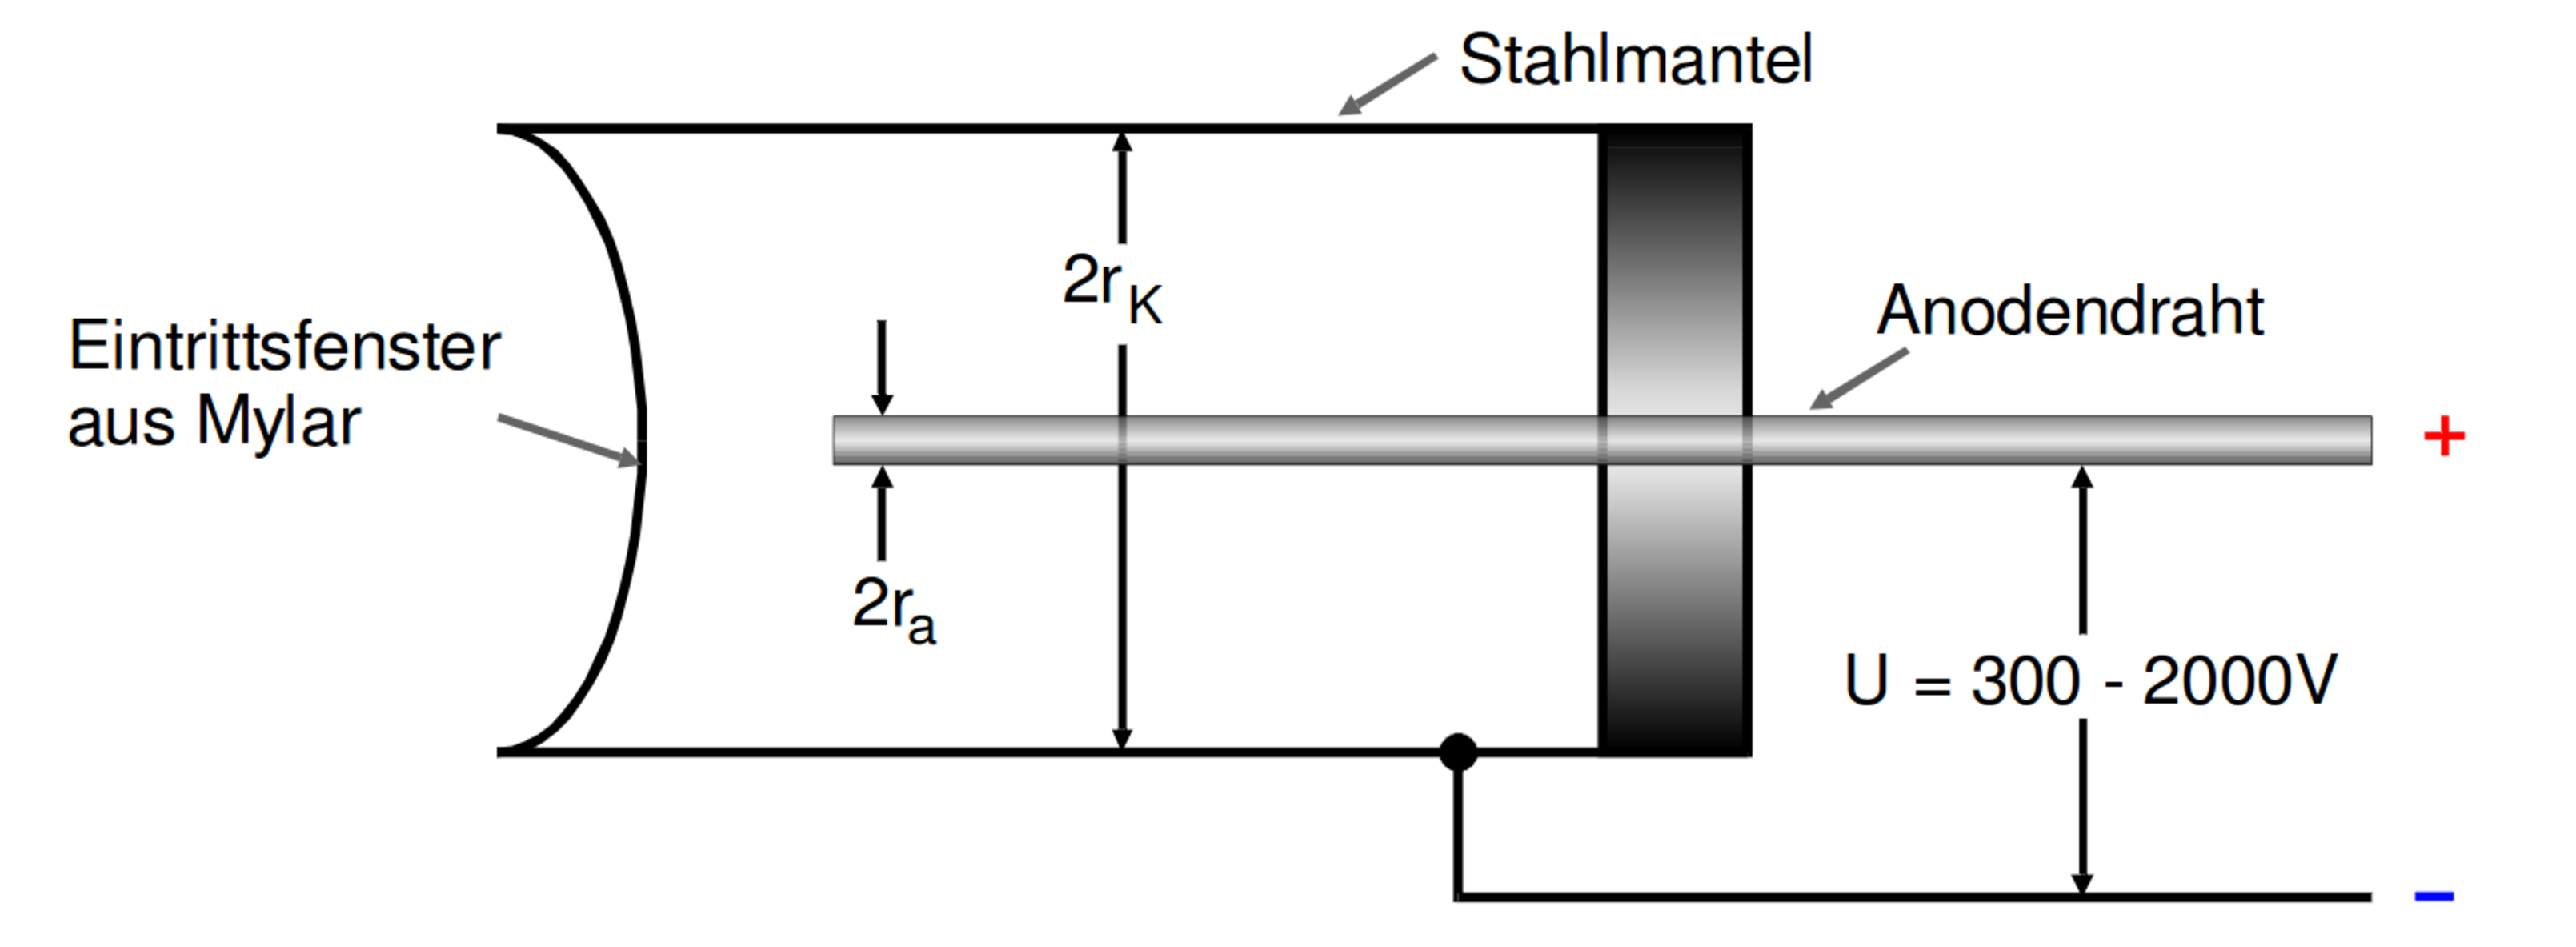
\includegraphics[height=4cm]{picture/Skizze.pdf}
  \caption{Aufbau eines Geigermüllerzählrohr \cite{sample}}
  \label{fig:skizze}
\end{figure}
Zwischen dem Anodendraht und dem Stahlmantel wird eine äußere Spannungangelgt, wodurch eine radialsymetrisches Feld zwischen Annodendraht und Kathode entsteht, deren Feldstärke 
\begin{equation}
  E(r) = \frac{U}{r ln \frac{r_\text{k}}{r_\text{a}}}
  \label{eqn:feld}
\end{equation}
beträgt. Der Stahlzilinder ist mit einem Gasgemisch aus Argon und Etyhlakohol gefüllt und wird Mylar-Folie verschlossen. Die beimischung des Alkohols soll die Nachentladung auf welche im weiteren Verlauf noch weiter eingegangen wird unterdrücken werden. Durch die Wahl von Mylar-Folie als Stirnfenster soll die Abschirmung von $\alpha$ verhindert werden und diese somit für das Geiger-Müllerzählrohr messbar seien.


\subsection{Fehlerrechnung}
Sämtliche Fehler und Fehlerfortpflanzungen werden mit Hilfe des Paketes "uncertainties" \cite{uncertainties} aus Python berechnet. Mit ausnahme des Fehlers der Zählrate, dieser wird über
\begin{align*}
	\Delta N = \frac{\sqrt{n_\text{Impulse}}}{\Delta t}
\end{align*}
berechnet. \\
Sämtliche Fits werden mit Hilfe der Paketes "lmfit" \cite{lmfit} aus Python berechnet.
